\documentclass[sigconf,anonymous,review]{acmart}

\usepackage{tikz}
\usepackage{booktabs}
\usepackage{graphicx}

\setcopyright{none}
\acmConference[Under review]{Under review}{}{}
\acmYear{2026}
\settopmatter{printacmref=false}
\renewcommand\footnotetextcopyrightpermission[1]{}
\makeatletter
\AtBeginDocument{%
  \fancypagestyle{standardpagestyle}{%
    \fancyhf{}%
    \fancyfoot[C]{\if@ACM@printfolios\footnotesize\thepage\fi}%
    \fancyhead[LO]{\ACM@linecountL\@headfootfont\shorttitle}%
    \fancyhead[RE]{\@headfootfont\@shortauthors\ACM@linecountR}%
    \fancyhead[LE]{\ACM@linecountL}%
    \fancyhead[RO]{\ACM@linecountR}%
  }%
  \pagestyle{standardpagestyle}%
}
\makeatother

\newtheorem{remark}{Remark}
\newtheorem{assumptionx}{A}
\newcounter{assumption}
\newenvironment{assumption}{\refstepcounter{assumption}\par\medskip\noindent\textbf{A\theassumption.}\enspace}{\par\medskip}
\newenvironment{assumptionstar}[1]{\par\medskip\noindent\textbf{#1.}\enspace}{\par\medskip}

\setlength{\emergencystretch}{3em}

\newcommand{\E}{\mathrm E}
\newcommand{\iidsiminline}{{\scriptstyle\stackrel{\mathrm{iid}}{\sim}}}
\newcommand{\iidsim}{{\stackrel{\mathrm{iid}}{\sim}}}
\newcommand{\ind}{\perp\!\!\!\perp}
\newcommand{\R}{\mathrm{I}\!\mathrm{R}}
\newcommand{\nn}{\nonumber}
\DeclareMathOperator{\var}{var}
\DeclareMathOperator{\cov}{cov}

\begin{document}

\title[EARL: Bipartite Experiments with Partial Assignment]{EARL: Exposure- and Allocation-Reweighted Linear Estimator for Bipartite Experiments with Partial Assignment}

\author{Alexey Kurennoy}
\affiliation{%
  \institution{}
  \city{}
  \country{}
}
\email{}

\begin{abstract}
Bipartite A/B tests are experiments in which treatment is randomised over one set of units, while outcomes are measured on another. For example, an online marketplace may test a new pricing algorithm on a random subset of \emph{items}, while the outcome of interest~--- say, purchase satisfaction~--- is measured on \emph{customers}, each of whom interacts with many items.

Existing methods for analysing bipartite experiments assume that every randomisation (diversion) unit is assigned to either treatment or control. In practice, often only a subset participates in the experiment: platforms cap rollout risk, reserve holdout groups, and split their unit population across many concurrent tests. Ignoring the unassigned units biases estimation, while including them requires care.

We construct an unbiased linear estimator for bipartite experiments with partial assignment. We show that observations must be reweighted not only by the (centred) share of treated connections among the participating ones (i.e., the exposure) but also by the number of participating connections, each inverse-weighted by its participation propensity, so that units whose connections are well covered by the experiment carry proportionally more weight. The resulting estimator, EARL (Exposure- and Allocation-Reweighted Linear), is unbiased, consistent, and asymptotically normal; we devise two asymptotic variance estimators for it and show that it has minimal variance in a natural class of linear estimators. EARL remains unbiased \emph{regardless of the experience the unassigned units receive}, as long as they contribute to expected outcomes additively; in particular, they can be freely allocated to other, non-overlapping tests. Our theory is complemented with a simulation study on two public datasets, in which EARL attains up to six times lower error than the strongest existing baseline and, in some configurations, over an order of magnitude lower than Horvitz--Thompson-style alternatives.
\end{abstract}

\begin{CCSXML}
<ccs2012>
 <concept>
  <concept_id>10002950.10003648.10003662</concept_id>
  <concept_desc>Mathematics of computing~Probabilistic inference problems</concept_desc>
  <concept_significance>500</concept_significance>
 </concept>
 <concept>
  <concept_id>10002944.10011122.10002945</concept_id>
  <concept_desc>General and reference~Experimentation</concept_desc>
  <concept_significance>500</concept_significance>
 </concept>
</ccs2012>
\end{CCSXML}
\ccsdesc[500]{Mathematics of computing~Probabilistic inference problems}
\ccsdesc[500]{General and reference~Experimentation}

\keywords{A/B testing, bipartite experiments, interference, average treatment effect, partial assignment}

\maketitle

\section{Introduction}\label{sec:introduction}

Online platforms routinely evaluate changes through randomised experiments (A/B tests). The textbook design randomises the same units on which outcomes are measured. In many important applications, however, the intervention is applied to one population while its effects materialise on another. A marketplace changes the pricing mechanism of \emph{items}, but cares about the satisfaction of \emph{customers} who interact with those items; an advertising platform modifies the auction configuration of \emph{ad campaigns}, but measures the experience of \emph{users} exposed to many campaigns. Experiments of this kind are called \emph{bipartite}: one set of units~--- called \emph{randomisation} or \emph{diversion} units~--- is randomly split between treatment and control, while outcomes are recorded on a different set of \emph{analysis} (or \emph{outcome}) units, and the two sets are connected by a bipartite \emph{experiment graph} \cite{zigler2021bipartite,harshaw2023erl,doudchenko2020causal}. Because each analysis unit is typically connected to many randomisation units, its outcome depends on the whole profile of treatments among its connections; this dependence of each outcome on the treatments of many units invalidates the naive difference-in-means analysis and calls for dedicated estimators.

Existing methods for analysing bipartite experiments almost universally presume that \emph{every} randomisation unit is assigned to either treatment or control. Industrial reality is different: often only a subset of randomisation units participates in any given experiment \cite{kohavi2020trustworthy,tang2010overlapping}. There are at least three reasons: platforms limit the risk of changes by enrolling only a fraction (say, 20\%) of units; they run multiple concurrent experiments and sometimes divide the population of randomisation units between them, so that different tests ``own'' different slices; and holdout groups are often reserved for long-term measurement. In all these cases, the units left out of the experiment~--- we call them \emph{unassigned} or \emph{unallocated}~--- do not disappear: they remain connected to the analysis units through the experiment graph and keep influencing the measured outcomes. A customer's satisfaction depends on all items they interact with, not only on the items enrolled in our pricing test.

It is tempting to analyse such an experiment by simply deleting the unassigned units from the graph and applying a standard estimator to the reduced graph. This, however, produces a systematically \emph{biased} answer. The estimand of interest is the \emph{global average treatment effect} (GATE)~--- the change in average outcomes if the treatment were rolled out to \emph{all} randomisation units, compared with none. An estimator computed on the reduced graph does not ``know'' that each analysis unit has further, currently unassigned connections that will also switch to the treatment experience after the rollout; as we show in Section~\ref{subsec:estimator}, under the same linear-contributions model that makes EARL unbiased, the exposure-reweighted linear (ERL) estimator of \citet{harshaw2023erl} applied to the reduced graph converges to $q\cdot GATE$, where $q$ is the participation rate, thus having an attenuation of up to 90\% at realistic allocation rates. The problem is a special case of estimation under a misspecified interference graph, which is known to introduce bias that grows with the divergence between the assumed and true graphs \cite{weinstein2026causal,savje2024misspecified}. Inverse-probability-weighting (IPW) estimators, on the other hand, can be adapted to remain unbiased, but their weights (and with them the worst-case variance) grow exponentially in the number of connections, and the problem deteriorates further under partial assignment, because the probability of observing an extreme exposure shrinks geometrically with the participation rate.

In this paper, we show that for unbiased and practical estimation of the treatment effect under partial assignment, one has to weight the observations not only by the (centred) exposure of the respective analysis units but also by the inverse-propensity-weighted count of their participating connections, thereby tilting the estimator towards analysis units whose connections are well covered by the experiment while restoring, on average, each unit's full connectivity. We provide the exact recipe for this reweighting, yielding a novel ERL-type estimator we call EARL (Exposure- and Allocation-Reweighted Linear). We prove its unbiasedness, consistency, and asymptotic normality; devise estimators of its asymptotic variance, together enabling practical inference; and show that EARL has the smallest variance in a natural class of linear reweighting estimators, uniformly over the outcome models we consider.

The contributions of this paper are as follows.
\begin{itemize}
    \item \textbf{A novel unbiased estimator for bipartite experiments with partial assignment.} We construct an ERL-type estimator that is unbiased under partial assignment and remains ubiased \emph{whatever experience the unassigned units receive} (e.g., participation in other, non-overlapping experiments), as long as they contribute to the expected outcomes additively. It formally reduces to standard ERL at full assignment, and is provably the minimum-variance member of a natural class of linear estimators. We establish a bias bound without any linearity assumption, and exact unbiasedness, consistency, and asymptotic normality under a linear-contributions model.
    \item \textbf{Inference machinery.} We devise a closed-form, exactly unbiased estimator of EARL's variance in the spirit of \citet{harshaw2023erl}, and analyse the randomisation-inference variance estimator of \citet{shi2025scalableanalysisbipartiteexperiments} under partial assignment. For the latter, we identify a subtlety specific to partial assignment: the validity requires a null hypothesis stating that expected outcomes are unaffected by \emph{allocation} as well as assignment; we supply a full, self-contained proof under this null.
    \item \textbf{A reproducible semi-synthetic evaluation.} Following the experimental designs of \citet{doudchenko2020causal} and \citet{harshaw2023erl}, we benchmark EARL on a synthetic graph and on two public bipartite graphs (Amazon product reviews and MovieLens), varying the participation rate from 10\% to 100\%. EARL is unbiased in all linear-response scenarios and reduces the estimation error of the strongest existing baseline by up to a factor of six and that of Horvitz--Thompson alternatives, in some configurations, by more than an order of magnitude. We also map out, and explain, the low-allocation regime in which the biased reduced-graph estimator retains a lower total error.
\end{itemize}

All proofs are collected in the supplementary material available in the anonymised repository accompanying this paper.\footnote{\url{https://anonymous.4open.science/r/earl-code-CC51}}

\section{Related Literature}\label{sec:literature}

\textbf{Bipartite experiments.} The bipartite interference framework was formalised by \citet{zigler2021bipartite}, motivated by environmental applications in which interventions on power plants affect health outcomes in surrounding areas; see also \citet{hudgens2008toward,aronow2017estimating,eckles2017design} for the general treatment of interference in experiments. In online platforms, bipartite experiments arise in marketplaces and advertising systems, and a line of work addresses their design: correlation-clustering designs \cite{pouget2019variance}, exposure-optimised designs \cite{harshaw2023erl}, and cluster designs for one-sided randomisation \cite{brennan2022cluster}. \citet{bajari2021multiple} study multiple randomisation designs, which randomise both sides of the graph simultaneously. These design questions are orthogonal to ours; we take the (Bernoulli) design as given and focus on estimation when part of the population is not enrolled.

\textbf{Two families of estimators.} \emph{IPW (Horvitz--Thompson) estimators} build on exposure mappings \cite{aronow2017estimating}: outcomes are reweighted by the inverse probability of the observed exposure level; \citet{zigler2021bipartite} and \citet{doudchenko2020causal} develop this approach for bipartite structures, the latter using generalised propensity scores \cite{hirano2004propensity}. IPW requires minimal outcome-model assumptions, but the probability of a ``pure'' (all-treated or all-control) exposure decays geometrically in the number of connections, so the weights (and with them the worst-case variance) explode. \emph{ERL-type estimators} instead posit a response structure linear in the exposure: \citet{harshaw2023erl} introduce the exposure-reweighted linear (ERL) estimator and establish unbiasedness, asymptotic theory, and unbiased variance estimation; \citet{shi2025scalableanalysisbipartiteexperiments} make the pipeline scalable, add covariate adjustment (CA-ERL), and propose randomisation-based inference; \citet{lu2025design} give a design-based analysis with a conservative variance estimator. All of the above assume full assignment of the randomisation units.

\textbf{Partial participation.} Closest to our work, \citet{tan2025estimating} study bipartite experiments with \emph{partial eligibility}: a fixed, known subset of treatment-side units is eligible for randomisation, while the remaining units are never treated. They define total-effect estimands restricted to the eligible side (PTTE) and to spillovers on ineligible units (STTE), and estimate them with an ensemble of outcome models, generalised propensity scores, and machine-learning components, with bootstrap inference. Our setting differs in three substantive ways. First, in our framework participation itself is randomised (with probability $q$), which is common when an experimentation platform carves the population into slices for concurrent tests \cite{tang2010overlapping}; eligibility in \citet{tan2025estimating} is a deterministic attribute. Second, and more importantly, we make no assumption about what the unassigned units experience, for example, they may be exposed to \emph{other} interventions, as happens when they are allocated to concurrent experiments, whereas ineligible units in \citet{tan2025estimating} are never directly assigned treatment, although all units continue interacting and may be affected through spillovers. Third, our target is the classical GATE for a rollout to the \emph{whole} population, and our machinery is design-based with closed-form weights, exact unbiasedness, central limit theorems, and analytic variance estimators, rather than model-based ensembles with bootstrap uncertainty. The two approaches are thus complementary: theirs favours flexible outcome modelling under fixed eligibility, ours favours transparent, assumption-light inference under randomised partial assignment.

\textbf{Graph misspecification.} Running a full-assignment estimator on the reduced graph is equivalent to analysing the experiment under a misspecified interference graph. \citet{weinstein2026causal} bound the bias arising from misspecified interference networks and show it grows with the divergence between the assumed and true networks; \citet{savje2024misspecified} studies when misspecified exposure mappings still permit meaningful estimation. Our contribution can be seen as replacing an (incorrectly) reduced graph with a weighting scheme on the full graph that restores unbiasedness at a modest variance cost.

\section{Proposed Estimator}\label{sec:estimator}

\subsection{Problem Setup and Notation}\label{subsec:notation}

Let $\mathcal A$ and $\mathcal R$ be the populations of $N$ analysis and $M$ randomisation units, respectively, and let $\mathcal C\subset \mathcal A \times \mathcal R$ be the set of connections between them. Together, the triple $\langle \mathcal A,\,\mathcal R,\,\mathcal C\rangle$ forms a bipartite graph that is commonly referred to as the \emph{experiment graph}. In the literature, analysis units are also called \emph{outcome} or \emph{measurement} units, and randomisation units are also called \emph{diversion}, \emph{treatment}, or \emph{intervention} units \cite{zigler2021bipartite,harshaw2023erl,doudchenko2020causal,tan2025estimating}. In our running marketplace example, the randomisation units are items, the analysis units are customers, and a connection $(a,\,r)$ records that customer $a$ interacts with item $r$. We use $d_\mathcal{A}$ to denote the maximum number of randomisation units connected to a given analysis unit and $d_\mathcal{R}$~~---  the maximum number of analysis units connected to a given randomisation unit.

Randomisation units are allocated for participation in the experiment independently at random with probability $q\in(0,\,1)$. Let $\mathbf{S} =(S_1,\,\ldots,\,S_M)$ be the vector of allocation indicators: $S_r$ is 1 if the $r$-th randomisation unit participates in the experiment and $0$ otherwise, $S_r\iidsiminline \mathrm{Bernoulli}(q)$. Randomisation units participating in the experiment are randomly and independently assigned to the treatment group with probability $p\in(0,\,1)$. Let $\mathbf Z=(Z_1,\,\ldots,\,Z_M)$ be the vector of assignment indicators: $Z_r$ is 1 if the $r$-th unit is (or would be, should it participate) assigned to the treatment, $Z_r\iidsiminline \mathrm{Bernoulli}(p)$. In industrial experimentation systems both indicators are computed by deterministic hashing of unit identifiers \cite{tang2010overlapping,kohavi2020trustworthy}, so $Z_r$ is well defined (though immaterial) even for units that do not participate. We assume that allocation and assignment are performed independently of each other, i.e., $\mathbf S \ind \mathbf{Z}$. While existing methods for analysing bipartite experiments assume that all randomisation units are assigned (i.e., $q=1$), in this paper we consider the partial assignment case ($q < 1$). It means that we have three groups of randomisation units: unassigned ($S_r = 0$, expected count $(1-q)M$), treatment ($S_r=1$, $Z_r=1$, expected count $pqM$), and control ($S_r=1$, $Z_r=0$, expected count $(1-p)qM$).
Note that even though unassigned units do not participate in the experiment, they are still connected to analysis units via the experiment graph and influence the outcomes associated with analysis units.

For a given analysis unit $a\in\mathcal A$, let $Y_a$ be the outcome (random) variable (which we assume to be integrable) and let $e_a(\mathbf{s},\,\mathbf{z})$
be the expected outcome conditional on $\mathbf S = \mathbf s$ and $\mathbf Z = \mathbf z$, i.e.,
\begin{equation}\label{eq:ea}
    e_a(\mathbf{s},\,\mathbf{z}) = \E[Y_a\mid \mathbf{S} = \mathbf{s},\,\mathbf{Z}=\mathbf{z}],\quad \mathbf{s}\in \{0,\,1\}^M,\, \mathbf{z}\in \{0,\,1\}^M.
\end{equation}
Furthermore, for each $a\in\mathcal{A}$, define the function $\mu_a$ as follows,
\begin{eqnarray}\label{eq:ma}
    \mu_a(x,\,y) &=& \E_{S_r\iidsim \mathrm{Bern}(x),\,Z_r\iidsim \mathrm{Bern}(y),\,\mathbf S\ind \mathbf Z}[e_a(\mathbf S,\,\mathbf Z)]\nonumber\\
    &=& \sum_{\textbf{s},\textbf{z}\in \{0,\,1\}^M}\prod_{r=1}^Mx^{s_r}(1-x)^{1-s_r}y^{z_r}(1-y)^{1-z_r}e_a(\textbf{s},\,\textbf{z}),
\end{eqnarray}
$x,\,y\in[0,\,1]$, with the convention $0^0=1$. The function $\mu_a$ is the expected outcome of unit $a$ in a hypothetical experiment with allocation rate $x$ and treatment rate $y$; it is a polynomial in $(x,\,y)$ and thus infinitely differentiable. Finally, let the function $\mu$ be the average of $\mu_a$ over the population of analysis units $\mathcal{A}$, i.\,e.,
\begin{equation}\label{eq:mu}
    \mu(x,\,y) = \frac 1 N \sum_{a\in\mathcal{A}} \mu_a(x,\,y),\qquad x\in[0,\,1],\, y\in[0,\,1].
\end{equation}

The goal of the experimenter is to estimate the \emph{global average treatment effect},
\begin{equation}\label{eq:gate}
    GATE = \frac 1 N\sum_{a\in\mathcal A} \left(\mu_a(1,\,1) - \mu_a(1,\,0)\right) = \mu(1,\,1) - \mu(1,\,0),
\end{equation}
i.e., the contrast between average expected outcomes when \emph{all} randomisation units receive treatment and when all of them receive control. This is the quantity relevant for the launch decision: it describes the world after a full rollout.

In what follows, $\mathcal D(a)$ denotes the set of randomisation units that are connected to the analysis unit $a$, i.e.,
\begin{equation*}
    \mathcal{D}(a) = \{r\in\mathcal{R}\colon (a,\,r)\in \mathcal{C}\}.
\end{equation*}

All random variables are assumed to be defined on a common probability space $(\Omega,\,\mathcal F,\,\Pr)$. In all asymptotic statements, the design parameters $p$ and $q$ are held fixed as the number of units grows.

\subsection{Exposure- and Allocation-Reweighted Linear Estimator}\label{subsec:estimator}

Let $H_a$ be the so-called exposure of analysis unit $a$, i.e., the share of treated units among the randomisation units $a$ is connected to,
\begin{equation}\label{eq:Ha}
    H_a = \frac{1}{|\mathcal{D}(a)|}\sum_{r\in\mathcal{D}(a)} Z_r.
\end{equation}
When all randomisation units are assigned ($q=1$), the standard ERL estimator \cite{harshaw2023erl} is defined as the average of outcomes $Y_a$ weighted by the standardised exposures,
\begin{equation}{\label{eq:erl}}
    \hat\tau_{ERL} = \frac 1 N \sum_{a\in\mathcal A} \frac{H_a - \E[H_a]}{\var \left(H_a\right)}Y_a =\frac{1}{N}\sum_{a\in\mathcal A}\sum_{r\in\mathcal{D}(a)}\frac{Z_r - p}{p(1-p)}Y_a.
\end{equation}
As demonstrated in \cite{harshaw2023erl}, ERL is unbiased for GATE under a linear exposure-response assumption.

Under partial assignment ($q<1$) two additional quantities describe how well the experiment covers the connections of $a$. Let $G_a$ be the share of participating units among the connections of $a$ (the \emph{allocation coverage}),
\begin{equation}\label{eq:Ga}
    G_a = \frac{1}{|\mathcal{D}(a)|}\sum_{r\in\mathcal{D}(a)} S_r,
\end{equation}
and let $\tilde H_a$ be the exposure computed \emph{within} the participating connections,
\begin{equation}\label{eq:Hta}
    \tilde H_a = \frac{\sum_{r\in\mathcal{D}(a)} S_rZ_r}{\sum_{r\in\mathcal{D}(a)} S_r}\quad\textup{if } G_a>0.
\end{equation}
For isolated units ($\mathcal D(a)=\emptyset$) we set $H_a = G_a = 0$.
The estimator we propose weights each observation by the product of the allocation coverage and the centred within-experiment exposure, scaled by the inverse allocation rate:
\begin{eqnarray}\label{eq:earl}
    \hat \tau_{EARL} &=& \frac 1 N \sum_{a\in \mathcal A} |\mathcal D(a)|\,\frac{G_a\,(\tilde H_a - p)}{q\,p(1-p)}\, Y_a \nonumber\\
    &=& \frac 1 N \sum_{a\in \mathcal A} \sum_{r\in\mathcal{D}(a)}\frac{S_r}{q}\cdot\frac{Z_r - p}{p(1-p)}\, Y_a,
\end{eqnarray}
with the convention that the first form is $0$ whenever $G_a=0$ (as the second form makes explicit). We call it the Exposure- and Allocation-Reweighted Linear (EARL) estimator. In comparison with the standard ERL estimator \eqref{eq:erl}, EARL (i) computes exposures only over the connections actually enrolled in the experiment, and (ii) additionally tilts the weights towards those analysis units that have a high share of participating randomisation units among their connections, upweighting every participating connection by the inverse of its allocation propensity. Setting $q=1$ in \eqref{eq:earl} formally recovers ERL; throughout, we treat the partial-assignment case $q\in(0,\,1)$.

Three practical remarks are in order. First, EARL only requires the assignment indicators $Z_r$ of \emph{participating} units ($S_r=1$), which are always observed. Second, the weights depend only on design quantities ($q$, $p$) and the experiment graph, so the estimator is computable in a single $O(|\mathcal C|)$ pass over the graph edges, similarly to \cite{shi2025scalableanalysisbipartiteexperiments}. Third, as will be demonstrated in Section~\ref{subsec:analysis}, EARL is unbiased (and consistent) for GATE \eqref{eq:gate} \emph{regardless of the actual experience the unassigned units receive}~--- e.g., exposure to the treatment (a ``backtest'') or allocation to other, disjoint experiments~--- provided that experience enters the expected outcomes additively (Assumptions~A\ref{a:mu} and A\ref{a:4} below): the experimenter need not ensure that unassigned units keep receiving the control experience, and thus retains much greater experimentation throughput.

One natural way to apply the existing full-assignment machinery to GATE estimation under partial assignment is to ignore the presence of unassigned units, i.e., to exclude them and compute the standard ERL estimator \cite{harshaw2023erl} on the reduced graph,
\begin{equation}\label{eq:erl-drop}
    \hat \tau_{drop} = \frac 1 N \sum_{a\in\mathcal{A}}\sum_{r\in\mathcal{D}(a)}S_r\frac{Z_r-p}{p(1-p)}Y_a.
\end{equation}
Since the weights in \eqref{eq:erl-drop} differ from EARL's \eqref{eq:earl} exactly by the factor $1/q$, we have $\hat\tau_{drop} = q\,\hat\tau_{EARL}$ identically, so under the assumptions of Section~\ref{subsec:analysis} $\E[\hat\tau_{drop}] = q\cdot GATE$, \emph{whatever experience the unassigned units deliver}~--- the reduced graph does not ``know'' that the analysis units have further, currently unassigned connections (a worked example is given in Section~3.2 of the supplementary material).

The $1/q$ correction is, however, not ad hoc: the next proposition shows that among \emph{all} linear reweighting estimators that correct the allocation in an unbiased way, EARL is the most efficient, uniformly over the class of outcome models introduced in Section~\ref{subsec:analysis}. Consider the family
\begin{equation}\label{eq:class}
    \hat\tau_{c} = \frac 1 N \sum_{a\in \mathcal A} \sum_{r\in\mathcal{D}(a)}c(S_r)\,\frac{Z_r - p}{p(1-p)}\, Y_a,\qquad c\colon\{0,\,1\}\mapsto\R,
\end{equation}
which contains the reduced-graph ERL ($c(s)=s$), EARL ($c(s)=s/q$), and, e.g., the estimator with the standardised-allocation weight $c(s)=(s-q)/(q(1-q))$.

\begin{proposition}\label{prop:optimality}
    Let the experiment graph contain at least one connection ($\mathcal C\neq\emptyset$), and let Assumptions A\ref{a:1}, A\ref{a:mu}, and A\ref{a:no-autocorrelation} of Section~\ref{subsec:analysis} hold (the latter includes square integrability of the outcomes). Suppose, in addition, that the conditional second moments $m_a(\mathbf s,\,\mathbf z) := \E[Y_a^2\mid \mathbf S=\mathbf s,\,\mathbf Z=\mathbf z]$ exclude would-be assignments in the sense of Assumption~A\ref{a:mu}(ii): for every $a\in\mathcal A$, $m_a(\mathbf s,\,\mathbf z) = m_a(\mathbf s,\,\mathbf z')$ whenever $z_r=z_r'$ for all $r$ with $s_r=1$. Then:
    \begin{itemize}
        \item[\textup{(a)}] $\hat\tau_c$ satisfies $\E[\hat\tau_c]=\E[\hat\tau_{EARL}]$ for every outcome model satisfying the above if and only if $q\,c(1)=1$; in particular, under the conditions of Theorem~\ref{th:unbiasedness}(b) below, $\hat\tau_c$ is unbiased for GATE if and only if $q\,c(1)=1$;
        \item[\textup{(b)}] for every $c$ with $q\,c(1)=1$,
        \begin{equation*}
        \var(\hat\tau_c) = \var(\hat\tau_{EARL}) + c(0)^2\,\var(\hat\tau_U),
        \end{equation*}
        where $\hat\tau_U = N^{-1}\sum_{a}\sum_{r\in\mathcal D(a)}(1-S_r)\frac{Z_r-p}{p(1-p)}Y_a$. Consequently, $\var(\hat\tau_c) \ge \var(\hat\tau_{EARL})$, with equality if and only if $c(0)=0$ or $\var(\hat\tau_U)=0$.
    \end{itemize}
\end{proposition}

Like Assumption~A\ref{a:mu}(ii) itself, the second-moment condition holds under the standard randomisation construction, in which the assignment indicators are exogenous to all outcome disturbances and an unassigned unit's would-be assignment is never materialised. The proof (Section~A.2 of the supplementary material) rests on an exact orthogonal decomposition: any admissible $\hat\tau_c$ equals EARL plus a mean-zero term that is uncorrelated with it, so deviating from $c(0)=0$ can only add noise. The guarantee is confined to the class \eqref{eq:class}.

\subsection{Unbiasedness and Consistency}\label{subsec:analysis}

We begin by stating and discussing the assumptions we use to prove the unbiasedness of the EARL estimator \eqref{eq:earl}. The first assumption formalises the experimental design described in Section~\ref{subsec:notation}.

\begin{assumption}\label{a:1}
The allocation and assignment indicators satisfy $S_1,\,\ldots,\,S_M \iidsim \mathrm{Bernoulli}(q)$, $q\in(0,\,1)$, and $Z_1,\,\ldots,\,Z_M \iidsim \mathrm{Bernoulli}(p)$, $p\in(0,\,1)$, with the vectors $\mathbf S=(S_1,\ldots,S_M)$ and $\mathbf Z=(Z_1,\,\ldots,\,Z_M)$ independent of each other: $\mathbf S \ind \mathbf Z$.
\end{assumption}

Somewhat differently from \cite{harshaw2023erl}, we do not maintain a linear response assumption in the strict sense: outcomes $Y_a$ need not be linear in the exposure $\tilde H_a$ or the allocation coverage $G_a$~--- indeed, they need not even be measurable with respect to them. We instead impose (jointly) weaker conditions on the \emph{conditional expectations} of the outcomes, the first of which states that the expected outcome of an analysis unit depends only on the allocation and assignment of its direct connections, with would-be assignments of unassigned units immaterial.

\begin{assumption}\label{a:mu}
For every analysis unit $a\in\mathcal A$, the conditional expected outcome $e_a$ defined in \eqref{eq:ea} satisfies:
\begin{itemize}
    \item[\textup{(i)}] \textup{(locality)} $e_a(\mathbf s,\,\mathbf z) = e_a(\mathbf s',\,\mathbf z')$ whenever $s_r=s_r'$ and $z_r=z_r'$ for all $r\in\mathcal D(a)$;
    \item[\textup{(ii)}] \textup{(exclusion of would-be assignments)} $e_a(\mathbf s,\,\mathbf z) = e_a(\mathbf s,\,\mathbf z')$ whenever $z_r=z_r'$ for all $r\in\mathcal D(a)$ with $s_r=1$.
\end{itemize}
\end{assumption}

Part (i) rules out ``higher-order'' effects on the expected outcome that travel through the graph beyond direct connections~--- effects along the canonical ``M-structure'', in which a randomisation unit not connected to $a_1$ influences $Y_{a_1}$ through the behaviour of another analysis unit and the state of a shared connection (an illustration is given in the supplementary material). The assumption asserts that such feedback loops are absent, or negligible in practice, \emph{on average}: it constrains conditional means only, not the outcomes themselves. This is a bipartite analogue of the neighbourhood-interference assumptions standard in the literature \cite{aronow2017estimating,harshaw2023erl,shi2025scalableanalysisbipartiteexperiments}, and it is weaker than requiring $Y_a$ to be a function of the treatments in $\mathcal D(a)$. Part (ii) merely says that the treatment bucket a unit \emph{would have} received, had it participated, cannot influence outcomes when the unit does not participate. Since would-be assignments are never materialised (in a hash-based system they are never even computed for non-participants), (ii) holds under the standard randomisation construction in which the assignment indicators are exogenous to all outcome disturbances; we state it explicitly because the would-be indicators $Z_r$ are formally defined for all units, and Assumption~A\ref{a:1} alone does not rule out a dependence of the outcome distribution on them.


Under Assumption~A\ref{a:mu}, the function $\mu_a$ defined in \eqref{eq:ma} depends on $e_a$ only through its restriction to the coordinates in $\mathcal D(a)$: all other coordinates integrate out, and $\mu_a(x,\,y)$ is a polynomial in $(x,\,y)$ on $[0,\,1]^2$ (an explicit decomposition is given in Section~3.3 of the supplementary material).

The last assumption before we present our unbiasedness result specifies a linear structure for the conditional expected outcomes as functions of the allocation and assignment indicators.

\begin{assumption}\label{a:4}
For each analysis unit $a\in\mathcal{A}$, the conditional expected outcome $e_a$ defined in \eqref{eq:ea} is additive in the contributions of individual randomisation units: there exist coefficients $\beta^a_{r,\,j}\in\R$, $r=1,\,\ldots,\,M$, $j=0,\,1,\,2,\,3$, such that
\begin{equation*}
    e_a(\textbf{s},\,\textbf{z}) = \sum_{r=1}^M\left(\beta^a_{r,\,0}+\beta^a_{r,\,1}(1-s_r)+\beta^a_{r,\,2}s_rz_r+\beta^a_{r,\,3}s_r(1-z_r)\right)
\end{equation*}
for all $\textbf{s}\in\{0,\,1\}^M$ and $\textbf{z}\in\{0,\,1\}^M$.
\end{assumption}
Assumption~A\ref{a:4} says that the expected outcome of unit $a$ is a sum of contributions of randomisation units, each contributing one of three values according to its group: unassigned ($\beta^a_{r,\,0}+\beta^a_{r,\,1}$), treatment ($\beta^a_{r,\,0}+\beta^a_{r,\,2}$), or control ($\beta^a_{r,\,0}+\beta^a_{r,\,3}$). Crucially, unassigned and control units may have \emph{different} contributions: we do not assume that unassigned units deliver the control experience~--- they may, e.g., be allocated to other, non-overlapping experiments (experiments randomising disjoint sets of randomisation units). The coefficients may vary arbitrarily across $a$ and $r$, allowing rich effect heterogeneity, and A\ref{a:4} restricts conditional means only. (Under A\ref{a:mu}, the coefficients $\beta^a_{r,\,j}$, $j\ge 1$, of units $r\notin\mathcal D(a)$ can be taken to be zero.)

We are now in a position to show that the EARL estimator is unbiased.
\begin{theorem}\label{th:unbiasedness}
    Let the random variables $S_r,\,Z_r\colon\Omega\mapsto\{0,\,1\}$, $r=1,\,\ldots,\,M$, satisfy Assumption A\ref{a:1}. Suppose the random variables $Y_a$, $a\in\mathcal A$, are integrable and Assumption~A\ref{a:mu} is true. Let the function $\mu\colon[0,\,1]\times[0,\,1]\mapsto\R$ be defined by relations \eqref{eq:ea}--\eqref{eq:mu}.

    Then
    \begin{itemize}
    \item[\textup{(a)}] the estimator $\hat\tau_{EARL}$ defined by \eqref{eq:earl} and the global average treatment effect (GATE) defined by \eqref{eq:gate} satisfy the following bound,
    \begin{eqnarray}\label{eq:bound}
        \left|\E[\hat\tau^{\phantom{1}}_{EARL}] - GATE\right| \le \sup_{x,\,y\in(0,\,1)}\Bigg(\left|\frac{\partial^3\mu}{\partial x^2\partial y}(x,\,y)\right| \nn\\ {}+ \left|\frac{\partial^3\mu}{\partial  x\partial y^2}(x,\,y)\right|\Bigg),
    \end{eqnarray}
    \item[\textup{(b)}] if, in addition, Assumption A\ref{a:4} holds true, $\hat \tau_{EARL}$ is unbiased,
    \begin{equation}\label{eq:unbiasedness}
        \E[\hat\tau^{\phantom{1}}_{EARL}] = GATE.
    \end{equation}
    \end{itemize}
\end{theorem}

Part (a) quantifies the bias without any linearity assumption: the estimator's expectation and the GATE are both values of the mixed derivative $\partial^2\mu/\partial x\partial y$ at (possibly different) interior points, so the bias is controlled by the third derivatives of $\mu$~--- a measure of non-linearity of the response surface. Under the additive-contributions model these third derivatives vanish identically, giving part (b).

The consistency result below uses an extra assumption: once we condition on allocation and assignment, no systematic co-movement remains between the outcomes of different analysis units~--- all cross-unit dependence is channelled through $(\mathbf S,\,\mathbf Z)$.

\begin{assumption}\label{a:no-autocorrelation} The outcome variables $Y_a$, $a\in\mathcal A$, are square integrable (which makes the conditional moments below well defined) and, conditional on $(\mathbf S,\,\mathbf Z)$, the errors
\begin{equation}\label{def:epsa}
    \varepsilon_a = Y_a - e_a(\mathbf{S},\,\mathbf{Z}),\qquad a\in\mathcal{A},
\end{equation}
are uncorrelated:
\begin{equation*}
    \E[\varepsilon_a \varepsilon_{a'}\mid \mathbf{S},\,\mathbf{Z}] = \E[\varepsilon_a\mid \mathbf{S},\,\mathbf{Z}] \cdot \E[\varepsilon_{a'}\mid \mathbf{S},\,\mathbf{Z}]\quad \forall\,a\neq a'\in\mathcal{A}.
\end{equation*}
\end{assumption}

The next theorem demonstrates that EARL is consistent as long as the experiment graph is not too dense.
\begin{theorem}\label{th:consistency}
    Let the random variables $S_r,\,Z_r\colon\Omega\mapsto\{0,\,1\}$, $r=1,\,\ldots,\,M$, satisfy Assumption A\ref{a:1}. Suppose there exists $L>0$ such that $\E[Y_a^2] \le L$ for all $a\in\mathcal A$ (uniformly across all values of $N$). Let Assumptions~A\ref{a:mu}, A\ref{a:4}, and A\ref{a:no-autocorrelation} hold true.

    Then, if $d^{\phantom{1}}_{\mathcal{R}}d^3_{\mathcal{A}}=o(N)$, the EARL estimator defined in \eqref{eq:earl} is consistent for GATE \eqref{eq:gate},
    \begin{equation*}
        \hat\tau^{\phantom{1}}_{EARL} \stackrel{p}{\to} GATE\qquad \textup{as }N\to\infty.
    \end{equation*}
\end{theorem}

The sparsity requirement $d_{\mathcal R}^{\phantom{1}}d_{\mathcal A}^3=o(N)$ coincides with the corresponding condition for the full-assignment ERL estimator \cite[Theorem~4.2]{harshaw2023erl}: partial assignment affects only the constants in the mean-squared-error bound (through the factor $q^{-1}$ in the weights), not the admissible graph-density regime.

\subsection{Inference}\label{subsec:inference}
In this section, we prove the asymptotic normality of the EARL estimator and devise estimators for its asymptotic variance. This enables statistical testing and confidence intervals based on the EARL estimator.

\subsubsection{Asymptotic Normality}

To prove asymptotic normality we strengthen the decorrelation requirement of Assumption A\ref{a:no-autocorrelation}, asking that the errors $\varepsilon_a$, $a\in\mathcal A$, defined in \eqref{def:epsa} be independent across observations and from the allocation and assignment indicators.

\begin{assumptionstar}{A\ref{a:no-autocorrelation}$^*$}
The errors $\{\varepsilon_a\}_{a\in\mathcal A}$, allocation indicators $\mathbf S$, and assignment indicators $\mathbf Z$ are jointly independent.
\end{assumptionstar}

Under A\ref{a:no-autocorrelation}$^*$, the products $\varepsilon_a\varepsilon_{a'}$ are automatically integrable ($\E[|\varepsilon_a\varepsilon_{a'}|] = \E[|\varepsilon_a|]\,\E[|\varepsilon_{a'}|]$), so the conditional uncorrelatedness required by Assumption~A\ref{a:no-autocorrelation} holds for merely integrable outcomes; since every result below that invokes A\ref{a:no-autocorrelation}$^*$ also bounds the fourth moments of the outcomes, Assumption~A\ref{a:no-autocorrelation} holds in full in all those settings.

The proof of asymptotic normality also relies on the following (and last) assumption of this subsection. It rules out practically irrelevant edge cases in which the GATE can be estimated at a faster than parametric rate. See the discussion in \cite[p.~475]{harshaw2023erl} for specific scenarios that are excluded by this condition.

\begin{assumption}\label{a:non-degeneracy} \textit{(Asymptotic Non-Degeneracy)} The normalised variance of the EARL estimator is bounded away from zero, i.e., there exists $\delta >0$ such that $N\cdot\var(\hat\tau_{EARL}) > \delta$ for all sufficiently large $N$.
\end{assumption}

\begin{theorem}\label{th:asymptotic-normality}
    Let the random variables $S_r,\,Z_r\colon\Omega\mapsto\{0,\,1\}$, $r=1,\,\ldots,\,M$, satisfy Assumption A\ref{a:1}. Suppose there exists $L>0$ such that $\E[Y_a^4] \le L$ for all $a\in\mathcal A$ (uniformly across all values of $N$) and Assumptions~A\ref{a:mu}, A\ref{a:4}, A\ref{a:no-autocorrelation}$^*$, and A\ref{a:non-degeneracy} are true.

    Then, if $d^{4}_{\mathcal{R}}d^{10}_{\mathcal{A}}=o(N)$, the EARL estimator defined in \eqref{eq:earl} is asymptotically normal,
    \begin{equation*}
        \frac{\hat\tau^{\phantom{1}}_{EARL} - GATE}{\sqrt{\var\left(\hat\tau^{\phantom{1}}_{EARL}\right)}}\stackrel{d}{\to} \mathcal{N}(0,\,1)\qquad \textup{as }N\to\infty.
    \end{equation*}
\end{theorem}

\subsubsection{Asymptotic Variance Estimation}\label{subsubsec:variance}
An estimator of the asymptotic variance of $\hat\tau^{\phantom{1}}_{EARL}$ can be constructed similarly to \cite[Section 5.1]{harshaw2023erl}. For that purpose, we will need a stronger version of Assumption~A\ref{a:4} under which the contributions of the randomisation units connected to a given analysis unit are homogeneous. Define the \emph{joint coverage--exposure} of unit $a$,
\begin{equation}\label{eq:Fa}
    F_a = \frac{1}{|\mathcal{D}(a)|}\sum_{r\in\mathcal{D}(a)} S_rZ_r = G_a\tilde H_a,
\end{equation}
the share of $a$'s connections that participate \emph{and} are treated (with $F_a=G_a=0$ if $\mathcal D(a)=\emptyset$).

\begin{assumptionstar}{A\ref{a:4}$^*$}
For every $a\in\mathcal A$ there exist $B^a_j\in\R$, $j=0,\,1,\,2$, such that
\begin{equation*}
    e_a(\mathbf s,\,\mathbf z) = B^a_0 + B^a_1 \, G_a + B^a_2 \, F_a ,
\end{equation*}
where $G_a$ and $F_a$ are evaluated at $(\mathbf s,\,\mathbf z)$.
\end{assumptionstar}

Assumption~A\ref{a:4}$^*$ is exactly the special case of Assumption~A\ref{a:4} in which the coefficients $\beta^a_{r,\,j}$ do not vary with $r$ within $\mathcal D(a)$ (and vanish outside), so it implies Assumptions~A\ref{a:mu} and~A\ref{a:4}. For an isolated unit the coefficients $B_1^a,\,B_2^a$ multiply identically zero quantities and are thus unidentifiable; we fix them at zero. With this convention, $\mu_a(x,\,y) = B_0^a + B_1^ax + B_2^axy$ and the unit-level effect is $\gamma_a := \mu_a(1,\,1)-\mu_a(1,\,0) = B_2^a$ for every $a\in\mathcal A$.

Let $\phi_a$ denote the EARL weight of unit $a$,
\begin{equation}\label{def:phi}
    \phi_a(\mathbf S,\,\mathbf Z) = \sum_{r\in\mathcal D(a)}\frac{S_r}{q}\cdot\frac{Z_r - p}{p(1-p)},
\end{equation}
so that $\hat\tau^{\phantom{1}}_{EARL} = N^{-1}\sum_{a\in\mathcal A}\phi_a(\mathbf S,\,\mathbf Z)Y_a$, and write $\hat\gamma_a = \phi_aY_a$ for the unit-level estimate. The variance of EARL decomposes into pairwise covariances, $\var(\hat\tau_{EARL}) = N^{-2}\sum_{a_1,a_2}\cov(\hat\gamma_{a_1},\hat\gamma_{a_2})$, and we estimate each covariance by a weighted product of the observed outcomes, $Y_{a_1}Y_{a_2}R_{a_1,a_2}$. Denote by
$$
\mathcal P = \{(a_1,\,a_2)\in\mathcal A^2\colon \mathcal D(a_1)\cap\mathcal D(a_2)\neq\emptyset\}
$$
the set of \emph{overlapping} pairs (including the diagonal). The weights $R_{a_1,\,a_2}$ are constructed as follows.
\begin{itemize}
    \item If $(a_1,\,a_2)\notin\mathcal P$, set $R_{a_1,\,a_2}=0$ (under Assumptions A\ref{a:1}, A\ref{a:mu}, and A\ref{a:no-autocorrelation}, such pairs have zero covariance).
    \item If $(a_1,\,a_2)\in\mathcal P$ and $a_1\neq a_2$, let $\mathbf m_{a_1,a_2}$ be the vector of the $8$ monomials
    \begin{equation*}
        (G_{a_1},\,F_{a_1},\,G_{a_2},\,F_{a_2},\,G_{a_1}G_{a_2},\,G_{a_1}F_{a_2},\,F_{a_1}G_{a_2},\,F_{a_1}F_{a_2}),
    \end{equation*}
    let $\Sigma_{a_1,a_2}$ be its $8\times 8$ covariance matrix under the design, and let $\mathbf c_{a_1,a_2} = \Sigma^{-1}_{a_1,a_2}\mathbf u$, where $\mathbf u$ is the coordinate vector selecting $F_{a_1}F_{a_2}$. Set
    \begin{equation}\label{def:R}
        R_{a_1,\,a_2} = \phi_{a_1}\phi_{a_2} - \mathbf c_{a_1,a_2}^{\top}\left(\mathbf m_{a_1,a_2} - \E[\mathbf m_{a_1,a_2}]\right).
    \end{equation}
    \item If $a_1=a_2=a$, apply the same construction with the $5$-dimen\-sional monomial vector $\mathbf m_{a,a} = (G_a,\,F_a,\,G_a^2,\,G_aF_a,\,F_a^2)$ and $\mathbf u$ selecting $F_a^2$:
    $R_{a,\,a} = \phi_{a}^2 - \mathbf c_{a,a}^{\top}(\mathbf m_{a,a} - \E[\mathbf m_{a,a}])$.
\end{itemize}
The rationale mirrors \cite[Section~5.1]{harshaw2023erl}: the first term of $R_{a_1,a_2}$ makes $Y_{a_1}Y_{a_2}\phi_{a_1}\phi_{a_2}$ an (automatically unbiased) estimator of $\E[\hat\gamma_{a_1}\hat\gamma_{a_2}]$, while the linear-in-monomials term is calibrated so that $Y_{a_1}Y_{a_2}\,\mathbf c^{\top}(\mathbf m-\E[\mathbf m])$ is an unbiased estimator of the product $\gamma_{a_1}\gamma_{a_2}=\E[\hat\gamma_{a_1}]\E[\hat\gamma_{a_2}]$ for \emph{all} values of the coefficients $B^a_j$; subtracting the two yields an unbiased estimator of the covariance. All the moments entering $\E[\mathbf m_{a_1,a_2}]$ and $\Sigma_{a_1,a_2}$ are polynomials in $p$, $q$ determined by $|\mathcal D(a_1)|$, $|\mathcal D(a_2)|$, and $|\mathcal D(a_1)\cap\mathcal D(a_2)|$; they can be computed in closed form before the experiment or estimated by Monte Carlo \cite{fattorini2006applying}. Theorem~\ref{th:asymptotic-variance} below assumes the exact design moments; Monte Carlo substitutes forfeit exact unbiasedness, and asymptotic validity then requires the number of independent auxiliary draws to grow fast enough for the error in $\Sigma^{-1}_{a_1,a_2}$ to remain negligible. Note that only pairs in $\mathcal P$ require any computation, so the estimator scales with the number of overlapping pairs (at most $Nd_{\mathcal A}d_{\mathcal R}$) rather than $N^2$.

The construction requires the matrices $\Sigma_{a_1,a_2}$ to be invertible, which we assume in a uniform manner.

\begin{assumption}\label{a:lambda0}
    There exists a sequence $\lambda_N>0$ such that for every pair $(a_1,\,a_2)\in\mathcal P$ the smallest eigenvalue of $\Sigma_{a_1,a_2}$ is at least $\lambda_N$, and $d^{3}_{\mathcal A}d^{3}_{\mathcal R} = o(N\lambda_N^2)$.
\end{assumption}

Assumption~A\ref{a:lambda0} is the analogue of the non-degenerate-exposures condition of \cite[Assumption~4]{harshaw2023erl} and, like it, can be verified by the experimenter before the experiment, since $\Sigma_{a_1,a_2}$ depends only on the design. Allowing $\lambda_N\to0$ is essential: the smallest eigenvalue of a diagonal pair's $\Sigma_{a,a}$ cannot exceed its $(G_a,\,G_a)$ entry $\var(G_a) = q(1-q)/|\mathcal D(a)|$, so a lower bound independent of $N$ would force bounded analysis-side degrees. The condition fails entirely, e.g., for analysis units with a single connection or pairs with identical connection sets; such pairs' covariance terms can be replaced by conservative upper bounds in the spirit of \cite[Proposition~5.2]{harshaw2023erl}, preserving asymptotic validity when the number of affected ordered pairs, weighted by the magnitude of the replaced terms, is $o(N)$.

Given the weights, the variance estimator is
\begin{equation}\label{def:hat-V}
    \hat V = \frac 1 {N^2} \sum_{a_1\in\mathcal A}\sum_{a_2\in\mathcal A} Y_{a_1}Y_{a_2}R_{a_1,\,a_2}.
\end{equation}

The following theorem demonstrates that $\hat V$ is exactly unbiased and can be used to perform inference based on $\hat\tau_{EARL}^{\phantom{1}}$.

\begin{theorem}\label{th:asymptotic-variance}
    Let the assumptions of Theorem~\ref{th:asymptotic-normality} hold with Assumption~A\ref{a:4}$^*$ in place of Assumptions~A\ref{a:mu} and A\ref{a:4} (in particular, $d^{4}_{\mathcal{R}}d^{10}_{\mathcal{A}}=o(N)$ and $\E[Y_a^4]\le L$), and let Assumption~A\ref{a:lambda0} hold. Let the variance estimator $\hat V$ be defined by \eqref{def:R}--\eqref{def:hat-V}.

    Then $\E[\hat V] = \var(\hat\tau^{\phantom{1}}_{EARL})$ for every $N$, $\hat V / \var(\hat\tau^{\phantom{1}}_{EARL})\stackrel{p}{\to} 1$ as $N\to\infty$, and
    $$
        \frac{\hat\tau^{\phantom{1}}_{EARL} - GATE}{\sqrt{\hat V}} \stackrel{d}{\to} \mathcal N(0,\,1).
    $$
\end{theorem}

Like its full-assignment counterpart, $\hat V$ can be negative in finite samples; Theorem~\ref{th:asymptotic-variance} implies $\Pr\{\hat V>0\}\to1$, and on the complementary event the studentised statistic may be defined arbitrarily, cf.\ \cite{harshaw2023erl}.

\subsubsection{Randomisation Inference}\label{subsubsec:ri}

An additional, computationally simpler variance estimator is available under a stronger null hypothesis. Specifically, consider
\begin{equation}\label{def:strong-null}
    H_0^*\colon\qquad e_a(\mathbf s,\,\mathbf z)\ \textup{does not depend on }(\mathbf s,\,\mathbf z),\quad \forall\,a\in\mathcal A.
\end{equation}
The null $H_0^*$ states that neither the assignment \emph{nor the allocation} of any randomisation unit affects the expected outcome of any analysis unit; it implies the pointwise null of zero expected effects but is stronger, and the strengthening is necessitated by partial assignment: under a concurrent experiment the outcomes may co-vary with the allocation indicators $\mathbf S$ even when our treatment has no effect, and a re-randomisation procedure, which regenerates $(\mathbf S,\,\mathbf Z)$ independently of the observed outcomes, destroys precisely this co-variation. Theorem~\ref{th:randomisation-inference} below uses $H_0^*$ together with Assumption~A\ref{a:no-autocorrelation}$^*$: constant conditional means and errors independent of the design together render the outcomes independent of $(\mathbf S,\,\mathbf Z)$. We demonstrate this effect numerically in Section~\ref{sec:simulations}.

The randomisation-inference methodology follows \cite[Section~4]{shi2025scalableanalysisbipartiteexperiments}: we re-randomise the allocation and assignment indicators, forming $J$ independent samples,
\begin{equation}\label{def:S-Z-samples}
    \begin{array}{c}
        \tilde{\mathbf{S}}_j = (\tilde S_{1,\,j},\ldots,\tilde S_{M,\,j}) \quad \iidsim \quad \mathrm{Bernoulli}(q),\\
        \tilde{\mathbf Z}_j = (\tilde Z_{1,\,j},\ldots,\tilde Z_{M,\,j}) \quad \iidsim \quad \mathrm{Bernoulli}(p),\\
        \tilde{\mathbf{S}}_j\ind \tilde{\mathbf Z}_j,
    \end{array}\qquad j=1,\,\ldots,\,J,
\end{equation}
drawn independently of the experimental data. Let $\hat\tau^{\phantom{1}}_{EARL}(\tilde {\mathbf S}_j,\,\tilde{\mathbf Z}_j)$ be the EARL estimator computed using the $j$-th generated sample of allocation and assignment indicators with the weight function \eqref{def:phi}, i.e.,
$$
    \hat\tau^{\phantom{1}}_{EARL}(\tilde {\mathbf S}_j,\,\tilde{\mathbf Z}_j) = \frac 1 N \sum_{a\in\mathcal{A}}\phi_a(\tilde {\mathbf S}_j,\,\tilde{\mathbf Z}_j)Y_a,\qquad j=1,\,\ldots,\,J.
$$
Note that these ``copies'' of the estimator are still computed using the same observed outcomes $Y_a$; only the allocation and assignment indicators are replaced with the re-randomised values.

Using the above notation, the randomisation-inference estimator of the variance of $\hat\tau^{\phantom{1}}_{EARL}$ is the empirical variance of the copies,
\begin{equation}\label{def:hatV}
    \hat V_{RI} = \frac{1}{J} \sum_{j=1}^J\left(\hat\tau^{\phantom{1}}_{EARL}(\tilde {\mathbf S}_j,\,\tilde{\mathbf Z}_j)-\frac 1 J\sum_{j'=1}^J\hat\tau^{\phantom{1}}_{EARL}(\tilde {\mathbf S}_{j'},\,\tilde{\mathbf Z}_{j'})\right)^2.
\end{equation}
We complete our theoretical development with a theorem demonstrating that $\hat V_{RI}$ can be used for significance testing based on $\hat\tau^{\phantom{1}}_{EARL}$. The validity proof for the analogous full-assignment procedure in \cite{shi2025scalableanalysisbipartiteexperiments} was found to have a flaw; our proof (Section~A.7 of the supplementary material) is self-contained.

\begin{theorem}\label{th:randomisation-inference}
    Let Assumptions A\ref{a:1}, A\ref{a:mu}, A\ref{a:no-autocorrelation}$^*$, and A\ref{a:non-degeneracy} hold, and suppose there exists $L>0$ such that $\E[Y_a^4] \le L$ for all $a\in\mathcal A$ (uniformly across all values of $N$). Let the strong null \eqref{def:strong-null} hold true, let $d^{4}_{\mathcal{R}}d^{10}_{\mathcal{A}}=o(N)$, and let the number of re-randomisations $J=J_N$ grow so that $d^{6}_{\mathcal{A}}d^{2}_{\mathcal{R}}=o(J_N)$. Let $\hat V_{RI}$ be defined by \eqref{def:S-Z-samples}--\eqref{def:hatV}.

    Then $\hat V_{RI} / \var(\hat\tau^{\phantom{1}}_{EARL})\stackrel{p}{\to} 1$ as $N\to\infty$, and
    for any $\alpha\in(0,\,1)$,
    \begin{equation*}
        \Pr\left\{\left|\hat\tau^{\phantom{1}}_{EARL}\right| > z_{1-\alpha/2}\sqrt{\hat V_{RI}}\right\}\to \alpha \qquad \textup{as }N\to\infty,
    \end{equation*}
    where $z_{1-\alpha/2}$ is the quantile of the standard normal distribution of level $1-\alpha/2$.
\end{theorem}

\section{Simulation Study}\label{sec:simulations}

We evaluate EARL in a semi-synthetic simulation study designed to stay close to the empirical evaluations of \citet{doudchenko2020causal} and \citet{harshaw2023erl}, while introducing partial assignment with allocation rates $q$ ranging from 10\% to 100\%. The full code, together with instructions reproducing every number and figure in this section, accompanies the paper.\footnote{The code, together with the supplementary document containing the full proofs, is available in an anonymised repository: \url{https://anonymous.4open.science/r/earl-code-CC51}.} As in any simulation-based evaluation, the data-generating processes are stylised. We mitigate this by building the experiment graphs from real datasets, whose degree distributions are far from any convenient parametric form, and by including scenarios that \emph{violate} our assumptions, but the results should be read as controlled evidence with a known ground truth rather than as a substitute for field validation.

\subsection{Setup}\label{subsec:sim-setup}

\textbf{Graphs.} We use three bipartite graphs (Table~\ref{tab:graphs}). \emph{Synthetic}: the design of \cite[Section~6.1]{doudchenko2020causal} ($N=1000$ analysis units, $M=100$ randomisation units, each analysis unit connected to $m_a\sim U\{1,\ldots,10\}$ randomisation units at random). \emph{Amazon}: the user--item graph built from Amazon product-review data \cite{he2016ups,mcauley2015image}, subsampling $N=1000$ users with 2--50 reviews, similarly to \cite[Section~6.2]{doudchenko2020causal}; items are randomisation units, mirroring an experiment that changes an item-level mechanism and measures customer satisfaction \cite{harshaw2023erl}. \emph{MovieLens}: the full MovieLens-100K user--movie graph \cite{harper2015movielens}, a deliberately dense stress case ($d_{\mathcal A}=737$) far outside our sparsity conditions.

\begin{table}
\caption{Experiment graphs used in the simulation study.}
\label{tab:graphs}
\begin{tabular}{lrrrrr}
\toprule
Graph & $N$ & $M$ & $|\mathcal C|$ & $d_{\mathcal A}$ & $d_{\mathcal R}$\\
\midrule
Synthetic & 1000 & 100 & 5415 & 10 & 76\\
Amazon & 1000 & 2718 & 3273 & 42 & 18\\
MovieLens & 943 & 1682 & 100000 & 737 & 583\\
\bottomrule
\end{tabular}
\end{table}

\textbf{Outcome models.} Outcomes follow $Y_a = e_a + \varepsilon_a$ with $\varepsilon_a\iidsiminline\mathcal N(0,\,\sigma_\varepsilon^2)$, $\sigma_\varepsilon^2 = 0.5$, as in \cite{doudchenko2020causal} (here and below the second argument of $\mathcal N$ denotes the variance) and
\begin{equation*}
    e_a = \alpha_a + \beta_a F_a + \gamma_u (1-G_a),
\end{equation*}
where $F_a$ is the joint coverage--exposure \eqref{eq:Fa} and the term $\gamma_u(1-G_a)$ captures the effect of unassigned connections (e.g., their participation in a concurrent experiment). The GATE equals $N^{-1}\sum_a\beta_a$. Following \cite[Section~8]{harshaw2023erl}, coefficients are drawn once and then held fixed across replications: \emph{S1} (positive heterogeneous effects) $\alpha_a\sim\mathcal N(-1,\,3/8)$, $\beta_a\sim\mathcal N(2,\,1)$; \emph{S2} (near-zero effects) $\alpha_a\sim\mathcal N(2,\,3/8)$, $\beta_a\sim\mathcal N(0,\,1/2)$; \emph{S3} (non-linear response, violating A\ref{a:4}) $e_a = \alpha_a + 4F_a(F_a-1)+\gamma_u(1-G_a)$ with $\alpha_a\sim\mathcal N(0,\,1/8)$ and $GATE=0$. Each scenario is run with $\gamma_u=1$ (unassigned units carry a concurrent-test effect), and S1 and S2 also with $\gamma_u=0$ (unassigned units deliver the control experience).

\textbf{Estimators.} We compare: \emph{EARL} \eqref{eq:earl}; \emph{ERL-drop} \eqref{eq:erl-drop}, the standard ERL on the reduced graph; \emph{IPW-assign}, the Horvitz--Thompson full-/empty-exposure contrast \cite{aronow2017estimating,zigler2021bipartite} on the reduced graph with assignment-only propensities $p^{k_a}$, $(1-p)^{k_a}$ ($k_a$ the number of participating connections); and \emph{IPW-alloc}, the same contrast on the full graph with propensities $(qp)^{|\mathcal D(a)|}$, $(q(1-p))^{|\mathcal D(a)|}$ accounting for both allocation and assignment, in the spirit of \cite{tan2025estimating}. For each graph, scenario, and $q\in\{0.1,\,0.2,\ldots,\,1.0\}$ we run 1000 replications with $p=1/2$ and report bias, standard deviation, and RMSE.

\subsection{Results}\label{subsec:sim-results}

\begin{figure*}
\centering
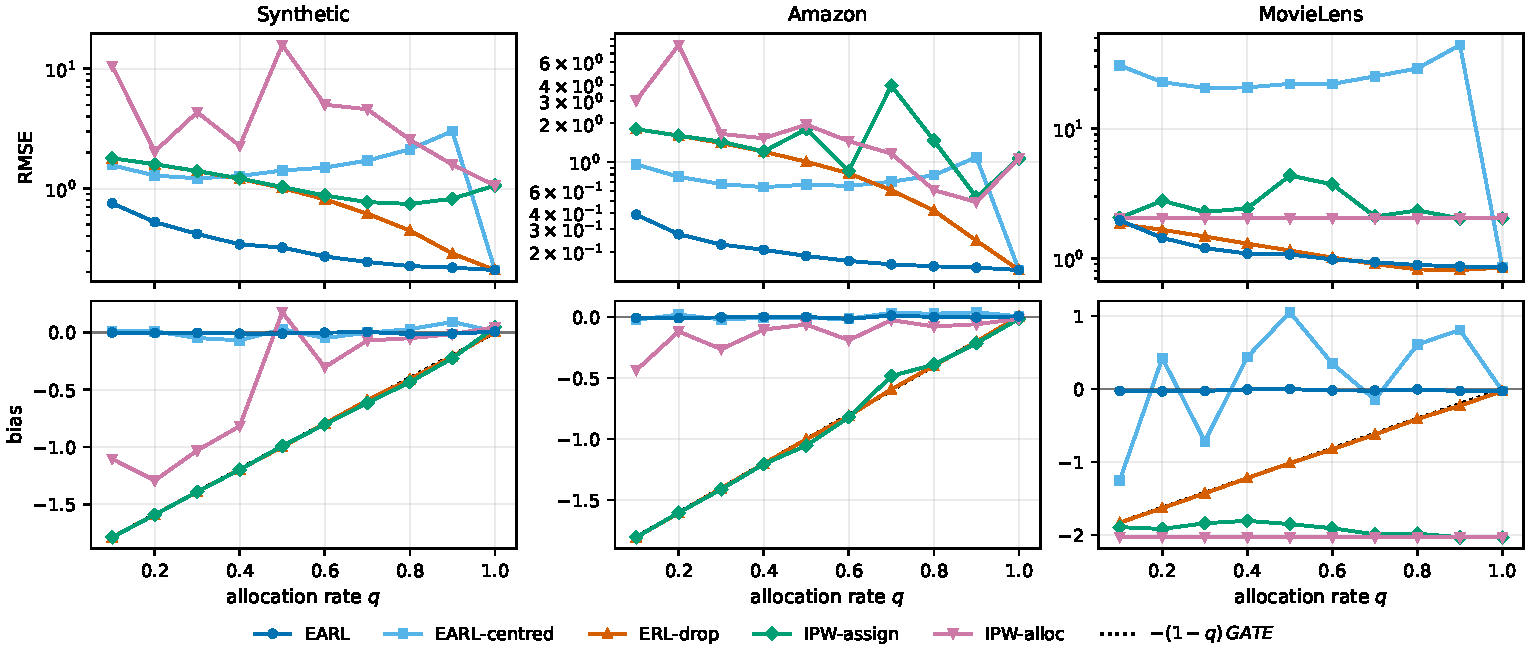
\includegraphics[width=0.8\textwidth]{figures/fig_rmse_bias.pdf}
\caption{RMSE (top, log scale) and bias (bottom) versus the allocation rate $q$ in scenario S1 ($\gamma_u=1$). EARL is unbiased everywhere and has the lowest RMSE at almost every allocation rate; ERL-drop has bias $-(1-q)\cdot GATE$; the IPW benchmarks are erratic or degenerate (IPW-alloc returns zero in every replication on MovieLens, where a pure exposure was never observed). At $q=1$, EARL and ERL-drop coincide with the standard ERL estimator.}
\label{fig:rmse-bias}
\end{figure*}

\begin{table*}
\caption{RMSE (with bias in parentheses) at allocation rates $q\in\{0.2,\,0.5,\,0.8\}$, scenario S1 with a concurrent-test effect on unassigned units ($\gamma_u=1$); 1000 replications, $p=0.5$. Best RMSE per column in bold. GATE $\approx 2.0$ in all three graphs.}
\label{tab:rmse}
\centering
\small\setlength{\tabcolsep}{4pt}\renewcommand{\arraystretch}{0.94}
\begin{tabular}{llccccccccc}
\toprule
& & \multicolumn{3}{c}{Synthetic} & \multicolumn{3}{c}{Amazon} & \multicolumn{3}{c}{MovieLens}\\
\cmidrule(lr){3-5}\cmidrule(lr){6-8}\cmidrule(lr){9-11}
Estimator & & $q=0.2$ & $q=0.5$ & $q=0.8$ & $q=0.2$ & $q=0.5$ & $q=0.8$ & $q=0.2$ & $q=0.5$ & $q=0.8$\\
\midrule
EARL & & \textbf{0.53} {\scriptsize$(-0.00)$} & \textbf{0.32} {\scriptsize$(-0.01)$} & \textbf{0.23} {\scriptsize$(-0.01)$} & \textbf{0.28} {\scriptsize$(-0.01)$} & \textbf{0.19} {\scriptsize$(-0.00)$} & \textbf{0.16} {\scriptsize$(-0.00)$} & \textbf{1.44} {\scriptsize$(-0.03)$} & \textbf{1.07} {\scriptsize$(-0.00)$} & 0.89 {\scriptsize$(-0.01)$}\\
ERL-drop & & 1.59 {\scriptsize$(-1.59)$} & 1.01 {\scriptsize$(-1.00)$} & 0.45 {\scriptsize$(-0.41)$} & 1.61 {\scriptsize$(-1.61)$} & 1.01 {\scriptsize$(-1.00)$} & 0.42 {\scriptsize$(-0.40)$} & 1.66 {\scriptsize$(-1.63)$} & 1.15 {\scriptsize$(-1.02)$} & \textbf{0.82} {\scriptsize$(-0.41)$}\\
IPW-assign & & 1.60 {\scriptsize$(-1.59)$} & 1.03 {\scriptsize$(-0.99)$} & 0.74 {\scriptsize$(-0.43)$} & 1.60 {\scriptsize$(-1.60)$} & 1.80 {\scriptsize$(-1.05)$} & 1.47 {\scriptsize$(-0.39)$} & 2.78 {\scriptsize$(-1.92)$} & 4.35 {\scriptsize$(-1.85)$} & 2.34 {\scriptsize$(-1.99)$}\\
IPW-alloc & & 2.04 {\scriptsize$(-1.29)$} & 15.79 {\scriptsize$(+0.18)$} & 2.56 {\scriptsize$(-0.05)$} & 8.13 {\scriptsize$(-0.12)$} & 1.95 {\scriptsize$(-0.06)$} & 0.61 {\scriptsize$(-0.08)$} & 2.03 {\scriptsize$(-2.03)$} & 2.03 {\scriptsize$(-2.03)$} & 2.03 {\scriptsize$(-2.03)$}\\
\bottomrule
\end{tabular}
\end{table*}

\textbf{Point estimation.} Figure~\ref{fig:rmse-bias} and Table~\ref{tab:rmse} summarise scenario S1, in which a genuine effect is present. First, EARL is unbiased at every allocation rate on all three graphs (largest absolute bias $0.03$, within Monte-Carlo error), while ERL-drop exhibits almost exactly the bias $-(1-q)\cdot GATE$ predicted by the theory~--- at $q=0.2$ it recovers barely a fifth of the true effect; IPW-assign inherits the same attenuation, and IPW-alloc, though unbiased in principle, is too noisy for its empirical mean to approach the target after 1000 replications. Second, EARL delivers the lowest RMSE in every cell of Table~\ref{tab:rmse} except one (MovieLens at $q=0.8$, where the biased ERL-drop edges it out), with the reduction relative to the strongest existing baseline reaching a factor of six on Amazon at low allocation rates ($0.28$ vs $1.61$ at $q=0.2$) and an order of magnitude relative to the IPW benchmarks. The IPW estimators illustrate the variance pathology that motivates ERL-type methods: on MovieLens (degrees in the hundreds) a fully treated or fully untreated neighbourhood was never observed, so IPW-alloc returned $0$ in every replication and IPW-assign is nearly degenerate; on sparser graphs their error is dominated by rare, enormous weights, and partial assignment amplifies the problem by shrinking the exposure propensities from $p^{|\mathcal D(a)|}$ to $(qp)^{|\mathcal D(a)|}$.

The $\gamma_u=0$ runs reveal the price of the $1/q$ reweighting. Since $\hat\tau_{EARL} = \hat\tau_{drop}/q$ under Bernoulli allocation, EARL's standard deviation is exactly $1/q$ times that of ERL-drop, and whether unbiasedness wins in RMSE depends on how this variance premium compares with the removed bias $(1-q)\cdot GATE$. The variance of both estimators is driven largely by the \emph{level} of the outcomes (the weights multiply $Y_a$, not a centred version of it): in S1 with $\gamma_u=1$ the concurrent-test term happens to offset the negative outcome intercept ($\E[\alpha_a]=-1$), so the level is small and EARL dominates broadly, as reported above; with $\gamma_u=0$ the level is of the order of the GATE itself, and on the synthetic ($q\le 0.2$) and MovieLens (all $q$) graphs the reduced-graph estimator's RMSE falls below EARL's, while on Amazon EARL still wins at every $q<1$ (by up to a factor of five). EARL remains unbiased throughout. The practical implication is standard: EARL should preferably be applied to outcomes centred by a fixed or pre-treatment baseline (cf.\ CA-ERL \cite{shi2025scalableanalysisbipartiteexperiments}); when the level cannot be reduced and $q$ is very small, the experimenter faces a genuine bias--variance choice. Our closed-form variance estimator makes this choice quantifiable before acting on the estimate: the two mean squared errors can be compared via the plug-in quantities $\hat V$ and $q^2\hat V + (1-q)^2\hat\tau^2_{EARL}$ (upward-biased by $(1-q)^2\var(\hat\tau_{EARL})$; substituting $\hat\tau^2_{EARL}-\hat V$ removes the excess at the price of possible negativity), so the shrunk estimator is indicated when the estimated effect is small relative to EARL's sampling noise.

In scenario S2 (effects indistinguishable from zero, $GATE\approx0.02$) the ranking reverses: ERL-drop's shrinkage bias is \emph{multiplicative} in the GATE, so with nothing to attenuate it attains the lowest RMSE among the non-degenerate estimators, whereas EARL pays the variance cost of unbiasedness. Two remarks are in order. First, the relative bias of ERL-drop is $100(1-q)\%$ of the estimand whatever its size: it wins on RMSE only when effects are near zero, and understates any consequential effect by the factor $q$. Second, using the reduced graph is rarely a deliberate choice~--- a pipeline that only sees the enrolled units reports $\hat\tau_{drop}$ with a confidence interval tightly centred on $q\cdot GATE$; once partial assignment \emph{is} modelled, EARL is available at no extra cost. In scenario S3 (non-linear response) the linear-response guarantees behind EARL and ERL-drop no longer apply and both exhibit visible bias, while the IPW contrasts remain unbiased in principle but are far too unstable to benefit from it; EARL's error decreases towards the ERL error as $q\to1$, and no method dominates. Full tables for S2, S3, and the $\gamma_u=0$ configurations are reproducible from the accompanying code.


\textbf{Randomisation inference.} We evaluate the randomisation-inference procedure of Section~\ref{subsubsec:ri} with all unit-level treatment effects equal to zero ($\beta_a\equiv 0$); the full table is in Section~B of the supplementary material. When the strong null $H_0^*$ holds exactly ($\gamma_u=0$), the empirical size of the nominal 5\% test is within Monte-Carlo error of the nominal level and $\hat V_{RI}$ matches the true variance (ratios $0.95$--$1.08$). When unassigned units carry a concurrent-test effect ($\gamma_u=1$), expected outcomes depend on $\mathbf S$ although all treatment effects are zero, and the variance ratio drifts up to $1.17$: re-randomisation reproduces the estimator's variance only under the allocation-inclusive null. Here the drift is conservative (the test under-rejects), but its direction is not guaranteed in general~--- hence Theorem~\ref{th:randomisation-inference} requires $H_0^*$; the closed-form $\hat V$ needs no null hypothesis, though it rests on the conditions of Theorem~\ref{th:asymptotic-variance}.

\section{Conclusion}\label{sec:conclusion}

We studied bipartite experiments in which only part of the randomisation-unit population is enrolled, a common regime on experimentation platforms. The standard practice of restricting the analysis to the enrolled units attenuates the estimated global treatment effect. To address this problem, we proposed EARL, an exposure- and allocation-reweighted linear estimator that removes this bias by upweighting every participating connection by its inverse allocation propensity. EARL is unbiased whatever (additively entering) experience the unassigned units receive, minimum-variance in its class, and consistent and asymptotically normal under the sparsity conditions known for full-assignment ERL. It is accompanied by two (closed-form and randomisation-inference) variance estimators. Simulations on real bipartite graphs confirm the theory, show up to six-fold accuracy gains over the strongest existing baseline, and delineate the low-allocation, high-outcome-level regime where outcome centring is advisable.

Several directions remain open: unit-specific design probabilities, covariate adjustment (in the spirit of CA-ERL \cite{shi2025scalableanalysisbipartiteexperiments}), and designs optimising the allocation split across concurrent experiments \cite{harshaw2023erl,brennan2022cluster}.


\section*{Ethical Considerations}
This paper develops statistical methodology for the analysis of randomised experiments and involves no data collection from human subjects. The empirical study uses two long-established public datasets (Amazon product reviews and MovieLens) solely to obtain realistic bipartite graph topologies; all outcomes are synthetically generated, and no personal or identifying information is used, inferred, or redistributed.

The method aims to improve measurement in experiments that platforms already run: unbiased effect estimates reduce the risk of shipping harmful or ineffective changes on the basis of systematically attenuated measurements. Two points nevertheless deserve attention. First, by making partially allocated experiments analysable without requiring unassigned units to receive the control experience, the method removes one obstacle to running more concurrent experiments; the safeguards for online experimentation (user consent frameworks, review processes, and harm monitoring) remain the operator's responsibility and are orthogonal to the choice of estimator. Second, like all reweighting estimators, EARL weights observations unevenly: analysis units whose connections are better covered by the experiment contribute more to the estimate. The weights depend only on design quantities (the experiment graph and the allocation and assignment probabilities), never on outcomes or on attributes of individuals, so the method itself introduces no disparate treatment; however, when effects are heterogeneous across subpopulations with systematically different connectivity, the estimand remains the population-level GATE, and practitioners should complement it with subgroup analyses before making decisions that may affect groups differently.

We foresee no security concerns or dual-use risks beyond those inherent in A/B-testing methodology in general.

\bibliographystyle{ACM-Reference-Format}
\bibliography{references}

\end{document}
